\documentclass[12pt]{article}
\usepackage[english]{babel}
\usepackage[utf8]{inputenc}
\usepackage{amsmath, amssymb, amsthm}
\usepackage{graphicx}
\usepackage{hyperref}
\usepackage[margin=.75in]{geometry}
\usepackage{xcolor}
\usepackage{tikz}

\setlength{\topmargin}{0pt}
\setlength{\headsep}{0pt}
\textheight = 600pt

\title{Graph Theory \\ Homework 7}
\author{Ben Kallus and Nicholas Adair}
\date{Due Monday, Monday, March 8}

\begin{document}
\maketitle

\noindent{\bf FIRST} Proposition: If $T$ is a tree, then $T$ contains at least $\Delta(T)$ leaves.
\begin{proof}
    Let $T$ be a tree.
    Let $v$ be a vertex of maximum degree in $T$, with neighbors $u_1, \hdots, u_{\Delta(T)}$.
    For each $i \in \{1,2,\hdots,\Delta(T)\}$, let $P_i = (v, u_i, \hdots, w_i)$ be a path of maximum length whose first edge is $vu_i$.

    Suppose, toward a contradiction, that there exists $i \in \{1,2,\hdots,\Delta(T)\}$ such that $w_i$ is not a leaf.
    Then, $w_i$ has a neighbor $x$ that is not its predecessor in $P_i$.
    Consider the walk $X$ obtained by appending $x$ to $P_i$.
    If $X$ is not a path, then it contains a cycle, so $T$ must not be a tree.
    On the other hand, if $X$ is a path, then it is longer than $P_i$, so $P_i$ must not be a path of maximum length whose first edge is $vu_i$.
    Thus, $w_i$ is a leaf for all $i \in \{1,2,\hdots,\Delta(T)\}$.

    Since $T$ is acyclic, each $P_i$ is a unique path with one shared vertex, $v$.
    Thus, each $w_i$ is unique.

    Thus, $T$ contains at least $\Delta(T)$ leaves.
\end{proof}

\newpage\noindent{\bf 4.2} Proposition: Every connected graph all of whose vertices have even degrees contains no bridges.
\begin{proof}
    Let $G$ be a connected graph all of whose vertices have even degrees.
    Suppose, toward a contradiction, that there exist $u,v \in V(G)$ such that $e=uv$ is a bridge in $G$.
    Let $G'$ be the component of $G-e$ containing $u$.
    Then, $u$ is the only odd vertex in $G'$.
    Thus, Corollary 2.3 has been violated, so it must be that $G$ has no bridges.
\end{proof}

\newpage\noindent{\bf 4.4} Proposition: If $G$ is a connected graph, and $e_1, e_2$ are distinct edges in $G$, then $G - e_1 - e_2$ has three components if and only if both $e_1$ and $e_2$ are bridges.
\begin{proof}
    Let $G$ be a connected graph.
    Let $e_1, e_2$ be distinct edges in $G$.

    Suppose that $G - e_1 - e_2$ has three components.
    Consider the following cases:

    {\bf Case 1.} Suppose that neither $e_1$ nor $e_2$ is a bridge.
    Then, $G-e_1$ is connected.
    Thus, $G-e_2$ has at most two components.

    {\bf Case 2.} Suppose without loss of generality that $e_1$ is a bridge, and $e_2$ is not.
    Then, $G-e_2$ is connected.
    Thus, $G-e_1$ has at most two components.

    Thus, it must be 

    Suppose $e_1$ and $e_2$ are bridges.
    Then, $G-e_1$ has two components, by the definition of a bridge.
    Let $G_1$ be the component of $G - e_1$ containing $e_2$.
    Then, by Theorem 4.1, $e_2$ is a bridge in $G_1$, since removing a vertex from a graph clearly does not introduce new cycles to that graph. % Should be said better.
    Thus, $G_1 - e_2$ has two components.
    Thus, $G - e_1 - e_2$ has three components.
\end{proof}

\newpage\noindent{\bf 4.6} Proposition: If $G$ is a connected graph of order $n \geq 3$ without bridges, and for every edge $e$ in $G$, each edge of $G-e$ is a bridge, then $G$ is a cycle graph.
\begin{proof}
    Let $G$ be a connected graph of order $n \geq 3$ without bridges such that for every edge $e$ in $G$, each edge of $G-e$ is a bridge.
    Then, by Theorem 4.1, every edge of $G$ participates in at least one cycle.
    Let $e \in E(G)$.
    Then, by Theorem 4.1, $G-e$ contains no cycles.
    Thus, $G-e$ is a tree.
    % Annoying to say, but obvious.
\end{proof}

\newpage\noindent{\bf 4.10}

{\bf (a)} $K_2 \cup K_1$.

{\bf (b)}
\begin{center}
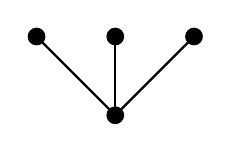
\begin{tikzpicture}
\draw[fill=black] (1, 0) circle (3pt);
\draw[fill=black] (0, 1) circle (3pt);
\draw[fill=black] (1, 1) circle (3pt);
\draw[fill=black] (2, 1) circle (3pt);

\draw[thick] (1, 0) -- (1, 1);
\draw[thick] (1, 0) -- (2, 1);
\draw[thick] (1, 0) -- (0, 1);
\end{tikzpicture}
\end{center}

{\bf (c)} Proposition: A tree $T$ containing exactly three vertices that are not end-vertices is a caterpiller.
\begin{proof}
    Let $T$ be a tree containing exactly three vertices $u,v,w$ that are not end-vertices.
    Since $u,v,w$ are the only vertices in $T$ that are not end-vertices, every end-vertex in $T$ must be connected to exactly one of $u,v,w$.
    Suppose that $\{uv, vw, wu\} \subseteq E(T)$. 
    Then $T$ contains the cycle $(u,v,w,u)$, so $T$ is not a tree.
    Thus, not all of $uv, vw, wu$ are edges in $T$.
    Now, suppose without loss of generality that neither $uv$ nor $vw$ is an edge in $T$.
    Then, since all vertices other than $u,v,w$ in $T$ are end-vertices, $v$ cannot be connected to either of $u,w$.
    Thus, $T$ is not connected, so $T$ is not a tree.
    Therefore, $T$ contains at least two of the edges $uv, vw, wu$.
    Thus, $T$ contains exactly two of the edges $uv, vw, wu$.
    Thus, the subgraph of $T$ induced by $\{u,v,w\}$ is $P_3$.
    Thus, since $u,v,w$ are the only vertices in $T$ that are not end-vertices, $T$ is a caterpiller.
\end{proof}

\newpage\noindent{\bf 4.14}
Applying Theorem 4.4 and the Handshaking Lemma,
\begin{align*}
    34 &= \frac{\sum\limits_{v \in V(T)} \deg(v)}2 \\
       &= \frac{25 \cdot 1 + 2 \cdot 2 + 3 \cdot 4 + 1 \cdot 5 + 2 \cdot 6 + 2 \cdot x}2 \\
       &= \frac{58+2x}2 \\
       &= 29 + x.
\end{align*}
Thus, $$x = 5.$$

\newpage\noindent{\bf 4.16}

{\bf (a)}
\begin{center}
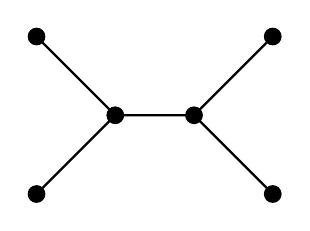
\begin{tikzpicture}
    \draw[fill=black] (0, 0) circle (3pt);
    \draw[fill=black] (1, 0) circle (3pt);
    \draw[fill=black] (2, 1) circle (3pt);
    \draw[fill=black] (2, -1) circle (3pt);
    \draw[fill=black] (-1, 1) circle (3pt);
    \draw[fill=black] (-1, -1) circle (3pt);

    \draw[thick] (-1,-1) -- (0,0) -- (1,0) -- (2,1);
    \draw[thick] (-1,1) -- (0,0);
    \draw[thick] (2,-1) -- (1,0);
\end{tikzpicture}
\end{center}

{\bf (b)}
Applying Theorem 4.4 and the Handshaking Lemma,
\begin{align*}
    2(n-1) &= \sum_{v \in V(T)} \deg(v) \\
           &= 3\left(\frac n3\right) + 1\left(\frac{2n}3\right) \\
           &= \frac53n.
\end{align*}
Thus, $$n=6.$$

Thus, the graph from (a) is the only tree in which two thirds of the vertices have degree 1 and the remaining one third of the vertices have degree 3.

\newpage\noindent{\bf 4.20}

{\bf (a)} Proposition: If $G$ is a graph of order $n$ and size $m$ with three cycles, then $m$ is not necessarily greater than or equal to $n+2$.
\begin{proof}
    Consider the following graph:
    \begin{center}
    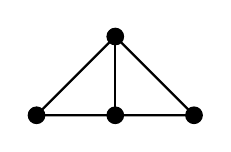
\begin{tikzpicture}
        \draw[fill=black] (0, 0) circle (3pt);
        \draw[fill=black] (1, 0) circle (3pt);
        \draw[fill=black] (2, 0) circle (3pt);
        \draw[fill=black] (1, 1) circle (3pt);

        \draw[thick] (0,0) -- (1,0) -- (2,0) -- (1,1) -- (0,0);
        \draw[thick] (1,0) -- (1,1);
    \end{tikzpicture}
    \end{center}
    Clearly, this graph has three cycles: the two inner triangles, and the outer triangle.
    However, it has 5 edges and 4 vertices, and $5 \not \geq 4+2$.
    Thus, in a graph of order $n$ and size $m$ with three cycles, $m$ is not necessarily greater than or equal to $n+2$.
\end{proof}

{\bf (b)} Proposition: There exist exactly two regular trees.
\begin{proof}
    Observe that $K_1$ is the only 0-regular tree, since it is the only connected 0-regular graph. % Probably needs better explanation.
    Observe that $K_2$ is the only 1-regular tree, since it is the only connected 1-regular graph. % Probably needs better explanation.
    Suppose that there exists a regular tree $T$ that is neither $K_1$ nor $K_2$.
    Then, $T$ is $n$-regular for some natural number $n \geq 2$.
    Since $T$ is $n$-regular, it contains only vertices of degree greater than or equal to 2.
    Thus, $T$ contains no leaves.
    However, by the result of the first proof in this assignment, $T$ contains at least $\Delta(T) = n$ leaves.
    Thus, $K_1$ and $K_2$ are the only regular trees.
\end{proof}

\newpage\noindent{\bf 4.24(a)}

    

\end{document}